\documentclass[a4paper, 12pt]{article}
\usepackage[utf8]{inputenc}
\usepackage[T1]{fontenc}
\usepackage[french]{babel}
\usepackage{graphicx}
\usepackage{amsmath}
\usepackage{amssymb}
\usepackage{geometry}
\geometry{hmargin=2.5cm,vmargin=1.5cm}
\usepackage{hyperref}

\pagestyle{headings}

\title{Projet OCaml}
\author{Wilfried LOCHUNGVU et Samuel MELENCHON \\ Groupe 10A}

\date{16 Mai 2021}

\begin{document}

\maketitle

\newpage


\tableofcontents

\newpage
\section{Tri par sélection V2}
\subsection{Fonctionnement}

Le tri par sélection v2 consiste à prendre la valeur la plus grande ou plus petite (selon comp choisi par l'utilisateur) et de la mettre en tête de liste, puis on continue ce processus sur le reste de la liste.

\subsection{Rapidité du tri}

On se sert de la fonction liste\_aleatoire afin de générer une liste aléatoire de x entiers limités à y.
On utilise également une fonction nous permettant d'obtenir le temps que met une fonction de trie à effectuer sa tâche.

On teste avec des listes aléatoires de plus de 175 valeurs ne dépassants pas 20.

~
\begin{center}
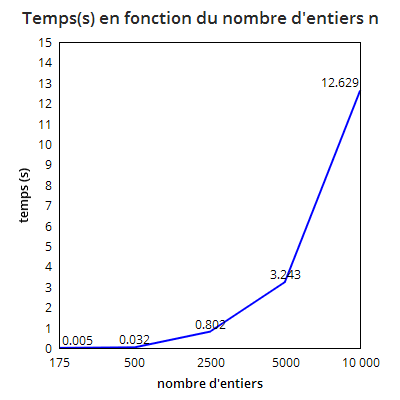
\includegraphics[scale=0.5]{triselN.png}
\end{center}
~

On en conclut donc que plus il y a d'éléments à traiter dans la liste, plus la fonction tri\_séléctionv2 met du temps a trier.

~

Maintenant on s'intéresse à la borne de la liste aléatoire. On teste avec des listes aléatoires de 100 entiers et on augmente progressivement la borne.

~

\begin{center}
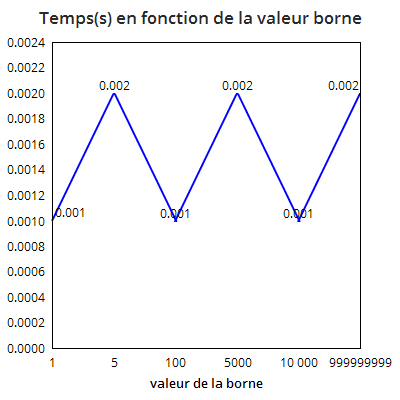
\includegraphics[scale=0.5]{triselB.png}
\end{center}
~

On remarque que peut importe la valeur de la borne lorsque le nombre d'entiers reste petit, la fonction reste régulière entre 0.001 et 0.002 secondes. 

Lorsqu'on augmente les deux paramètres progressivement on voit que le temps augmente considérablement.

\begin{table}[htbp]
  \centering
  \begin{tabular}{||l|c|r||}\hline
    \textbf{Nombre d'entiers} & \textbf{Borne} & \textbf{Temps (s)}\\\hline\hline
    100                     &    200                  & 0.00099999999999944578              \\\hline
    500                 & 700               & 0.030999999999998806                \\\hline
    2500                 & 4000             & 0.88299999999999557                 \\\hline
    5000                & 7000             & 3.3079999999999927  \\\hline
    10 000                 & 12 000         & 13.84899999999999 \\\hline
  \end{tabular}
  \label{tableausel}
\end{table}

~

Il semblerait donc que cette fonction soit beaucoup plus efficace sur des listes contenants une petite quantité de données non volumineuses à traiter.


\subsection{Complexité de la fonction}

Savoir le temps que met un algorithme à effectuer sa tâche n'est pas toujours significatif puisque d'un ordinateur à un autre, le temps peut changer selon plusieurs paramètres comme, la puissance de l'ordinateur, le langage... 

~

C'est pour cela qu'une ordre de grandeur notée O a été inventé, permettant d'obtenir une mesure fiable sur les algorithmes tout en calculant le nombre d'opérations qu'effectue l'algorithme. 

~

Ici, pour le tri par sélection, la fonction est d'ordre O(n), c'est-à-dire qu'il y aura n opérations à faire (n étant le nombre d'éléments dans la liste), par exemple : 

~

Trier [5,7,4]

~

\begin{itemize}
\item On va d'abord chercher le minimum qui est 4, et on le met dans une liste résultat [4].
\item Puis on cherche le minimum parmis [5,7] qui est 5 et on le met dans la liste résultat [4,5].
\item Et enfin il nous reste [7] qui est le minimum de la liste qu'on rajoute a [4,5,7].
\end{itemize}

~

Pour 3 éléments dans une liste nous avons effectué 3 boucles d'opérations, d'ou O(n).

~

C'est donc pour cela que la fonction tri\_selectionv2 est plus efficace sur des listes possédants peut de données peut importe les valeurs. 


\section{Tri du nain de jardin optimisé}

\subsection{Fonctionnement}

Le tri du nain consiste à trier par ordre croissant ou décroissant (selon le comparateur choisi par l'utilisateur) une liste. Pour cela il compare 2 éléments, si l'élément n est plus petit ou plus grand que l'élément n-1, alors il les échange, sinon il continue dans la liste tout en répétant ce processus.

\subsection{Rapidité du tri}

On va procéder de la même manière que la fonction tri\_seléctionv2 pour analyser sa rapidité.

On remarque que la fonction met très peu de temps (0. s) à trier des listes aléatoires d'environ moins de 55 éléments ne dépassants pas 20.

~

\begin{center}
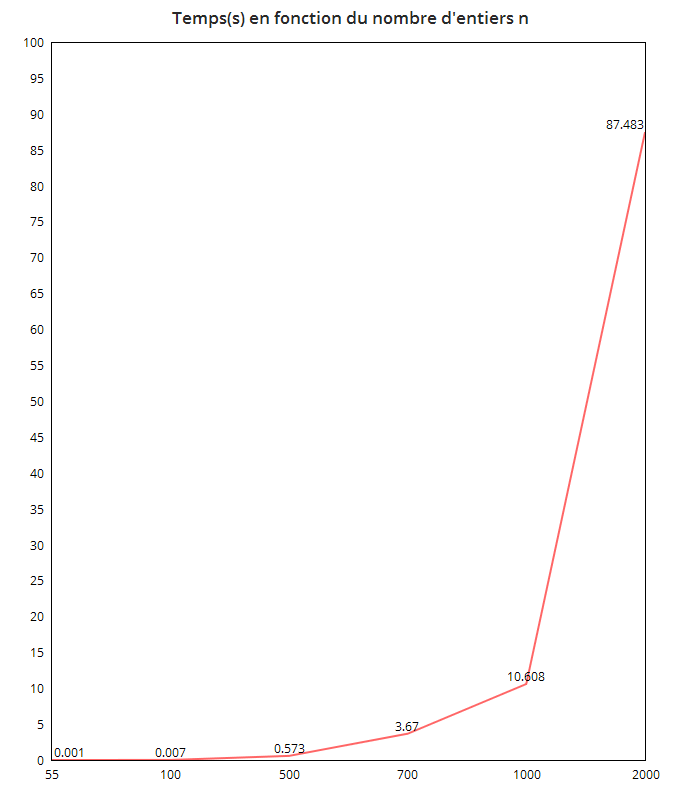
\includegraphics[scale=0.25]{tridunainN.png}
\end{center}
~

Comparée a tris\_selectionv2, tri\_du\_nain est plus lent. On peut voir que cette dernière met plus de temps.

~

\begin{center}
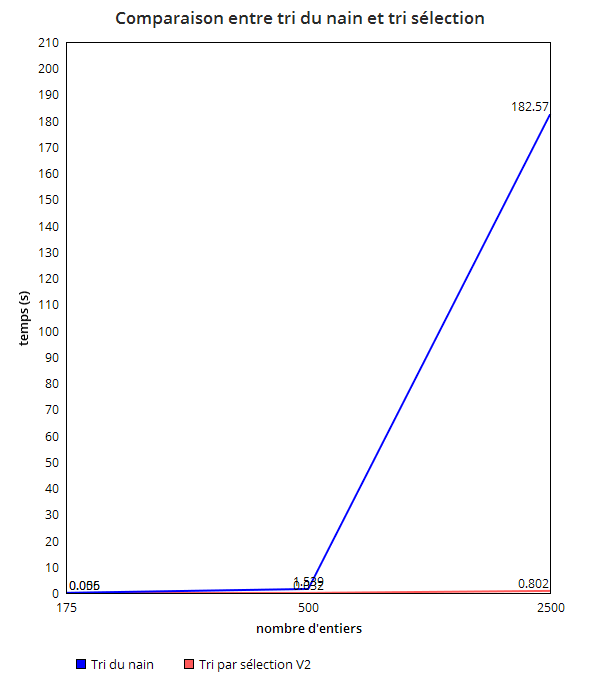
\includegraphics[scale=0.25]{trinainvstrisel.png}
\end{center}
~

Maintenant on va s'intéresser à la valeur que les éléments de la liste ne peuvent pas dépasser. On limite le nombre d'éléments aléatoires à 50.

~


\begin{center}
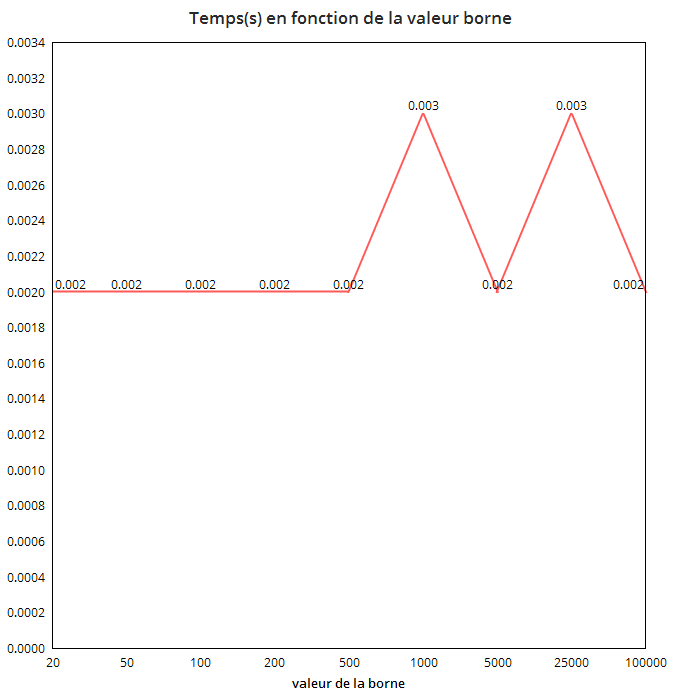
\includegraphics[scale=0.25]{tridunainborne.png}
\end{center}
~

On observe une fonction quasi constante (autour de 0.002 - 0.003 s) peut importe la valeur de la borne. La vitesse de la fonction est inférieure à celle de tri\_séléctionv2 si l'on modifie seulement la valeur de la borne.

~

Maintenant, on va modifier les deux paramètres de la fonction tri\_du\_nain progressivement.

~

\begin{table}[htbp]
  \centering
  \begin{tabular}{||l|c|r||}\hline
    \textbf{Nombre d'entiers} & \textbf{Borne} & \textbf{Temps (s)}\\\hline\hline
    100                     &    200                   &   0.014000000000010004            \\\hline
    500                 & 700               &   1.2530000000000427   \\\hline
    2500                 & 4000                 &   179.02800000000002               \\\hline
  \end{tabular}
  \label{tableaunain}
\end{table}

Si on compare ces résultats, on observe que la fonction tri\_du\_nain met beaucoup plus de temps que tri\_selection.
On observe donc que tri\_du\_nain est plus lente que tri\_sélectionv2.

\subsection{Complexité de la fonction}


Le tri du nain compare tous les éléments O(n) et fais une opération sur tous les éléments O(n). C'est pour cela qu'on dit qu'il est de type O(n^{2}). 

Cette fonction va donc mettre énormément de temps pour trier des listes peut importe la valeur des éléments. 



\section{Tri patience versions 1 et 2}

\subsection{Fonctionnement}

Les tris de patience consistent à trier les listes en mettant les éléments de la liste dans des listes tout en les triant en même temps. 

~

La v1, elle récupère les valeurs qui ont été mises dans une liste vide tout en la parcourant. 

~

La v2, elle fusionne toutes les listes presentes dans la liste afin d'en avoir qu'une seule. 

\subsection{Rapidité du tri\_patience\_v1}


On teste la fonction tri\_patience\_v1 avec des listes aléatoires de n entiers et de borne 20.

~


\begin{center}
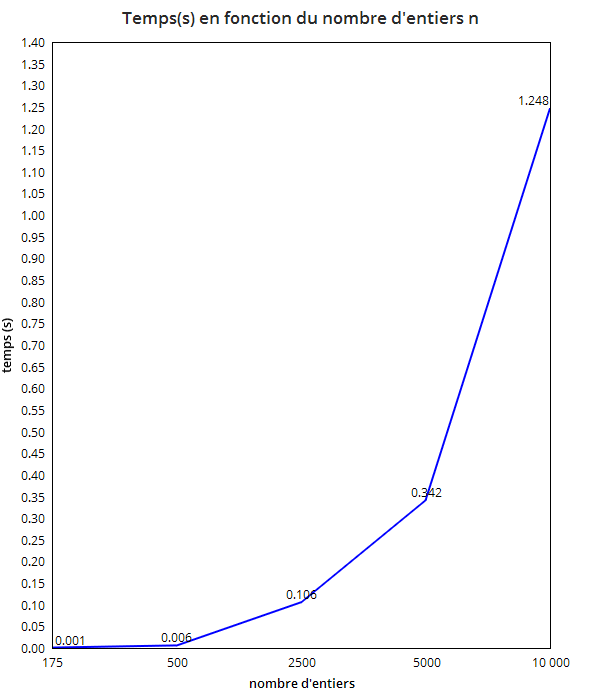
\includegraphics[scale=0.25]{tripat1N.png}
\end{center}
~

Si on compare avec les deux autres fonctions précédentes, tri\_patience\_v1 est nettement plus rapide que les autres lorsqu'elles varient selon n.

~

\begin{center}
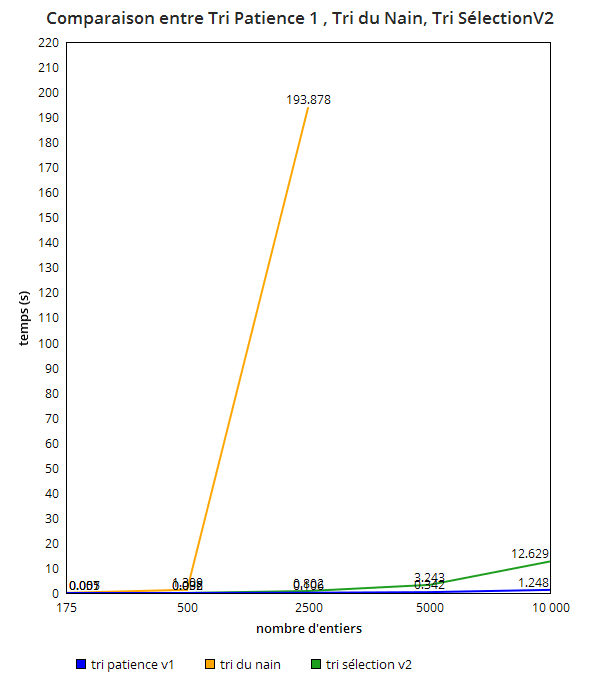
\includegraphics[scale=0.25]{tri_patience1-comparaisonN.png}
\end{center}
~

Maintenant, on teste la fonction tri\_patience\_v1 avec des listes aléatoires de 100 entiers et de borne y.

~


\begin{center}
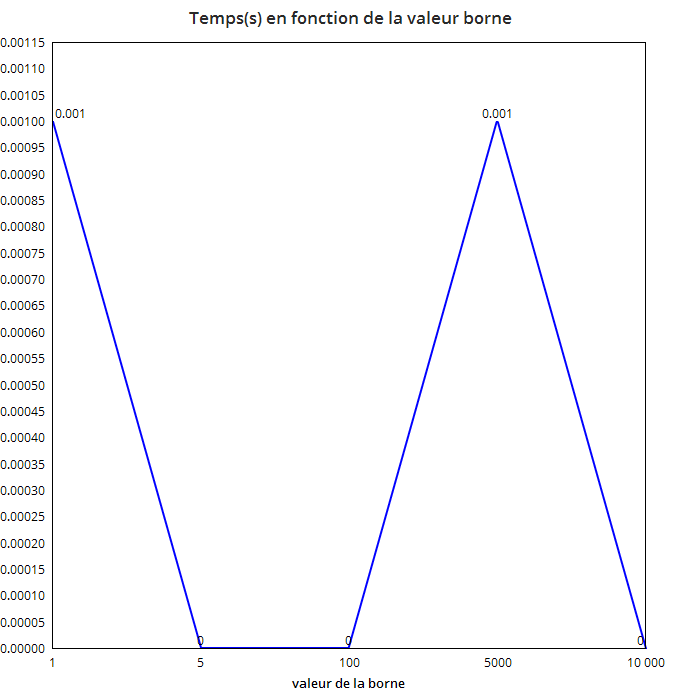
\includegraphics[scale=0.25]{tripat1B.png}
\end{center}
~

On observe que lorsque la valeur de la borne varie et que le nombre d'entiers reste constant, la vitesse de la fonction pour trier des listes varie entre 0. et 0.001 secondes. Si on compare avec les deux autres fonctions précédentes, on voit que tri\_patience\_v1 est nettement plus rapide que les autres. 

~


\begin{center}
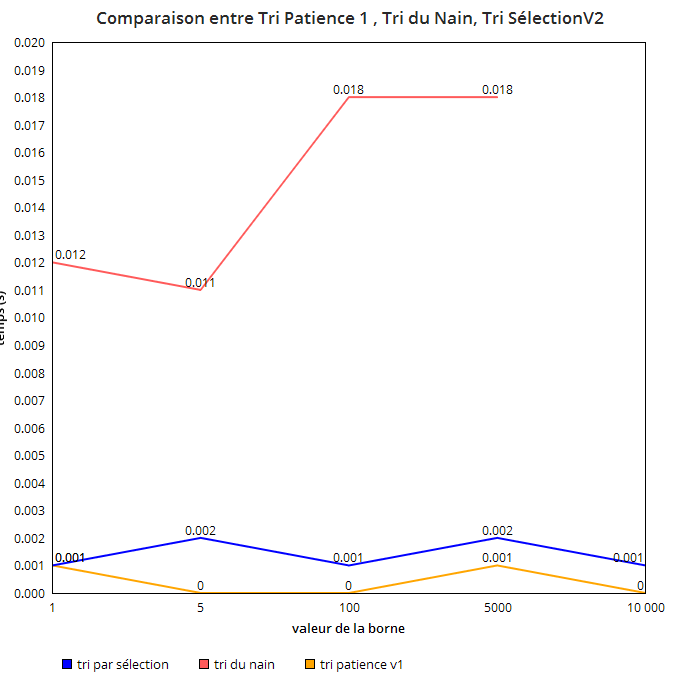
\includegraphics[scale=0.25]{tri_patience1_comparaisonB.png}
\end{center}
~

Maintenant on teste la fonction lorsque le nombre d'entiers et la borne varient. On observe des résultats beaucoup plus performants que les deux autres fonctions.
~

\begin{table}[htbp]
  \centering
  \begin{tabular}{||l|c|r||}\hline
    \textbf{Nombre d'entiers} & \textbf{Borne} & \textbf{Temps (s)}\\\hline\hline
    100                     &    200                  &   0.           \\\hline
    500                 & 700               & 0.0040000000000190994 \\\hline
    2500                 & 4000             & 0.04399999999998272    \\\hline
    5000                & 7000             & 0.11400000000003274  \\\hline
    10 000                 & 12 000         & 0.34100000000000819 \\\hline
  \end{tabular}
  \label{tablepat1}
\end{table}

\subsection{Rapidité du tri\_patience\_v2}

On teste la fonction tri\_patience\_v2 avec des listes aléatoires de n entiers et de borne 20.

~


\begin{center}
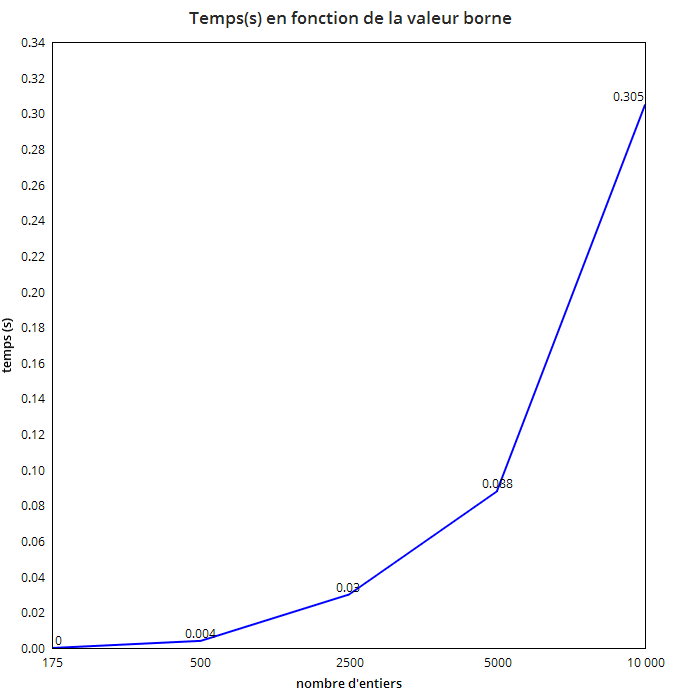
\includegraphics[scale=0.25]{trip2N.png}
\end{center}
~

Si on compare avec les trois autres fonctions précédentes, tri\_patience\_v2 est légèrement plus rapide que tri\_patience\_v1, et donc plus rapide que les autres lorsque n varie.

~

\begin{center}
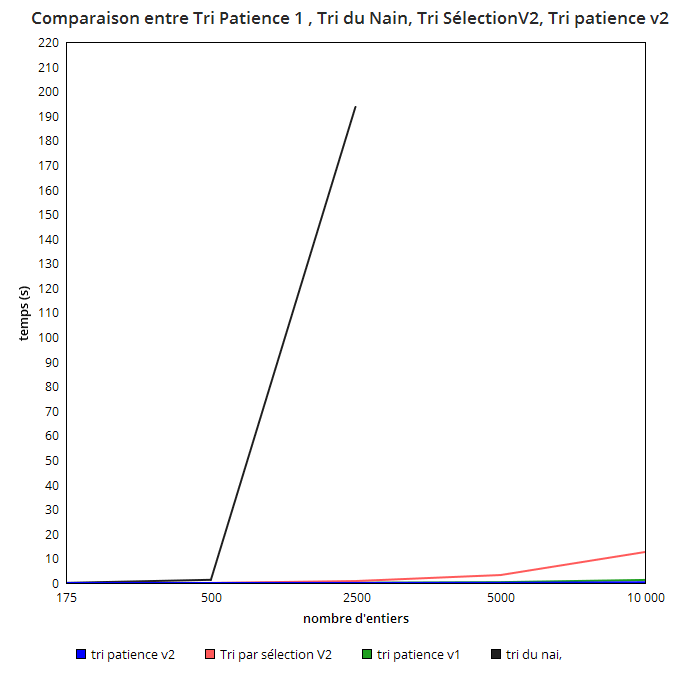
\includegraphics[scale=0.25]{tri_patience2_comparaisonN.png}
\end{center}
~

Maintenant, on teste la fonction tri\_patience\_v2 avec des listes aléatoires de 100 entiers et de borne y.

~

Pour les valeurs de n qui sont 1, 5, 100, 5000 et 10 000, la vitesse de la fonction est beaucoup plus proche de 0, par rapport aux autres fonctions, elle est plus rapide que les autres lorsque la borne varie.

~

Maintenant on teste la fonction lorsque le nombre d'entiers et la borne varient. tri\_patience\_v2 est beaucoup plus rapide que les trois autres fonctions.

\begin{table}[htbp]
  \centering
  \begin{tabular}{||l|c|r||}\hline
    \textbf{Nombre d'entiers} & \textbf{Borne} & \textbf{Temps (s)}\\\hline\hline
    100                     &    200                  &  0.            \\\hline
    500                 & 700               & 0.0010000000002037268 \\\hline
    2500                 & 4000             & 0.012999999999919964 \\\hline
    5000                & 7000             & 0.030000000000200089  \\\hline
    10 000                 & 12 000         & 0.081999999999879947 \\\hline
  \end{tabular}
  \label{tablepat2}
\end{table}



\subsection{Complexité de la fonction}











\section{Tri fusion}

\subsection{Fonctionnement}

Le tri fusion consiste à diviser la liste jusqu'à obtenir plusieurs morceaux de liste d'un seul élément afin des les comparer entre eux puis les "fusionner" afin de reconstituer une liste triée. 


\subsection{Rapidité du tri}

On teste la fonction tri\_fusion avec des listes aléatoires de n entiers et de borne 20.

~

\begin{center}
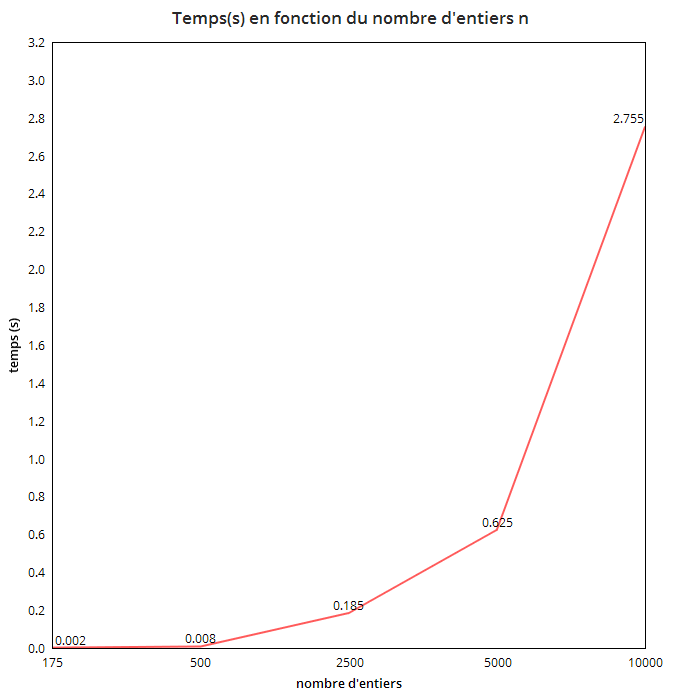
\includegraphics[scale=0.25]{trifusN.png}
\end{center}
~

Si on compare avec les quatre autres fonctions précédentes, tri\_fusion est moins rapide que tri\_patience\_v1 et tri\_patience\_v2, mais plus rapide que les deux autres fonctions.

~


\begin{center}
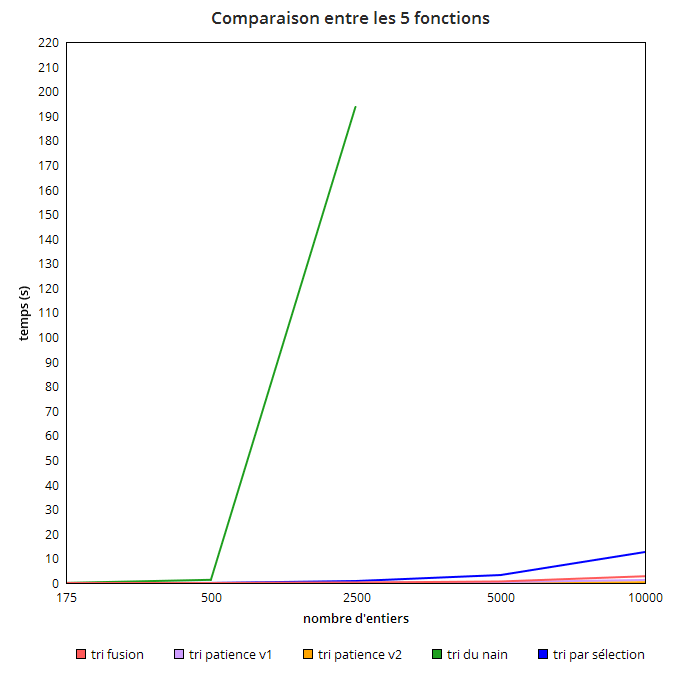
\includegraphics[scale=0.25]{tri_fusion_comparaisonN.png}
\end{center}
~

Maintenant, on teste la fonction tri\_fus avec des listes aléatoires de 100 entiers et de borne y.

~

Pour les valeurs de n qui sont 1, 5, 100, 5000 et 10 000, la vitesse de la fonction varie entre 0 et 0.001 secondes, comme tri\_patience\_v1.

~

Maintenant on teste la fonction lorsque le nombre d'entiers et la borne varient. tri\_fus est beaucoup plus rapide que les trois autres fonctions.


\begin{table}[htbp]
  \centering
  \begin{tabular}{||l|c|r||}\hline
    \textbf{Nombre d'entiers} & \textbf{Borne} & \textbf{Temps (s)}\\\hline\hline
    100                     &    200                  & 0.00099999999974897946  \\\hline
    500                 & 700               &  0.0079999999998108251\\\hline
    2500                 & 4000             & 0.14800000000013824 \\\hline
    5000                & 7000             &  0.63200000000006185 \\\hline
    10 000                 & 12 000         & 2.8179999999997563 \\\hline
  \end{tabular}
  \label{tablepat2}
\end{table}




\subsection{Complexité de la fonction}


En divisant la liste par 2 plusieurs fois de suite, on remarque un logarithme de base 2. 
Puis lorsqur l'on compare les différents éléments, on le fait n fois, en combinant donc les deux, on obtient O(n log n). 

Ce qui prouve que le tri fusion est très efficace. 



\section{Recherche d'éléments dans une
liste triée}



\subsection{Recherche dichotomique}

\subsection{Fonctionnement}
Dans la recherche dichotomique,le principe est de comparer l'élement central de la liste avec l'élement donné par l'utilisateur.
Trois possibilité s'offre donc a nous :
\begin{itemize}
    \item  Soit ils sont égaux et alors le programme est terminé.
    \item Soit l'élement centrale est plus grand que l'élément de l'utilisateur, ainsi on suppose que cet élement se trouve dans la premiere moitié du tableau.
    \item Soit l'élement centrale est plus petit que l'élement de l'utilisateur, alors on en déduit que cet élement se trouve dans la deuxieme moitié et ainsi de suite jusqu'à savoir si cette élemetn se trouve ou non dans le tableau
\end{itemize}

\subsection{Rapidité de la fonction}

On teste la fonction recherche\_dichotomique en faisant varier le nombre d'éléments dans la liste. On fixe la borne des éléments à 100 ainsi que 100 pour la borne max de la valeur recherchée.

~
\begin{center}
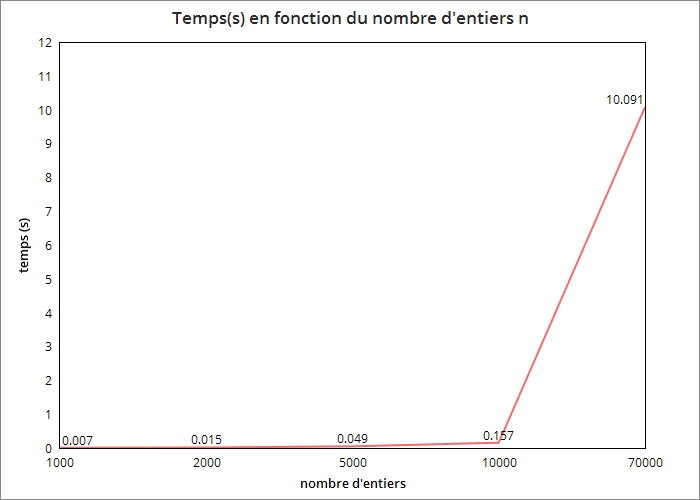
\includegraphics[scale=0.25]{recherchedichoN.png}
\end{center}
~

On remarque qu'a partir d'environ 87000 éléments dans la liste, la fonction est limitée au niveau du temps (trop de temps).

~

On teste maintenant la fonction recherche\_dichotomique en faisant varier la borne des éléments dans la liste. On fixe le nombre des éléments à 5 000 ainsi que 500 pour la borne max de la valeur recherchée.

~
\begin{center}
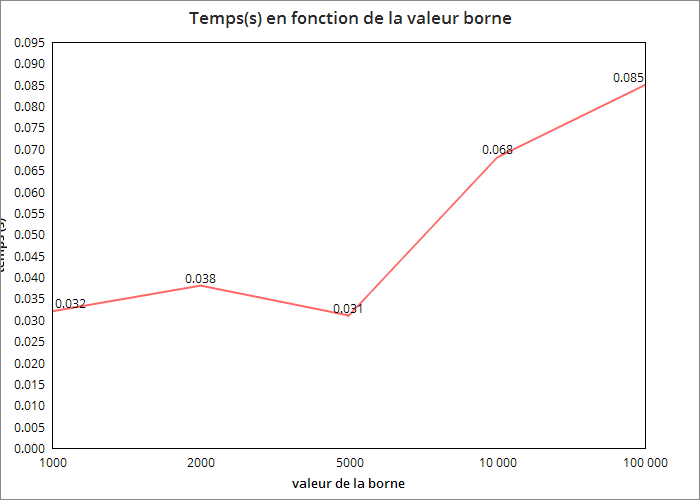
\includegraphics[scale=0.25]{recherchedichoM.png}
\end{center}
~

A partir de 5 000 pour la valeur de la borne, il arrive que la fonction mette beaucoup plus de temps que d'habitude (0.03 secondes / 0.08 secondes en moyenne), la vitesse ne peut être calculer car l'élément recherché n'est peut etre pas dans la zone à rechercher.

~

On teste maintenant la fonction recherche\_dichotomique en faisant varier la borne maximale de recherche des éléments dans la liste. On fixe le nombre des éléments à 5 000 ainsi que 500 pour la borne des éléments.

~
\begin{center}
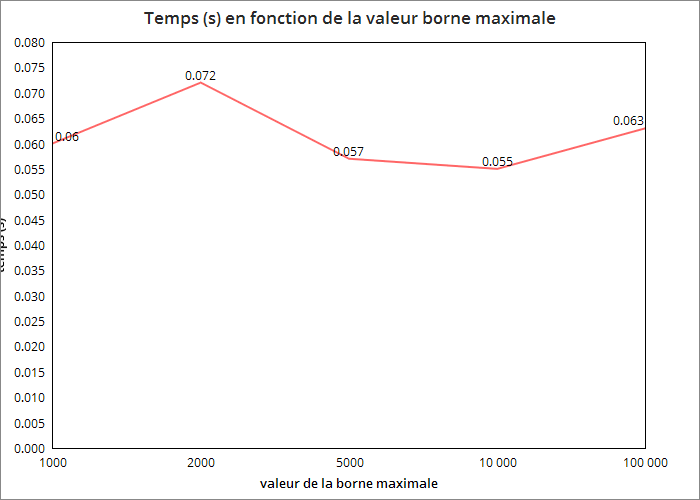
\includegraphics[scale=0.25]{recherchedichoBMAX.png}
\end{center}
~

On observe que la fonction varie entre 0.07 et 0.05 secondes.

~

Maintenant on teste la fonction lorsque tous les paramètres varient. recherche\_dichotomique.


\begin{table}[htbp]
  \centering
  \begin{tabular}{||l|c|r||}\hline
    \textbf{Nombre d'entiers} & \textbf{Borne BorneMaxRecherche} & \textbf{Temps (s)}\\\hline\hline
      5000           &  2500  3000      & 0.057999999999992724 \\\hline
    10 000           & 5000  6000       & 0.25400000000013279 \\\hline
    50 000           & 25 000  12 000   & 1.9949999999998909 \\\hline
    75 000          & 50 000  30 000    & 3.6520000000000437   \\\hline
  \end{tabular}
  \label{tablerechdich}
\end{table}




\subsection{Recherche séquentielle}

\subsection{Fonctionnement}
La recherche sequentielle,consite à prendre une liste trié et un élément afin de voir si cet élement en question est dans la liste. On obtiendra une réponse vrai ou fausse, suivant si l'élement est ou n'est pas dans la liste.
\subsection{Rapidité de la fonction}



\section{Conclusion}
\end{document}

